\documentclass[11pt]{article}

\newcommand{\yourname}{Cole Vick}
\newcommand{\yourcollaborators}{}

\def\comments{1}

%format and packages

\usepackage{graphicx}
%\usepackage{algorithm, algorithmic}
\usepackage{algpseudocode}
\usepackage{amsmath, amssymb, amsthm}
\usepackage{enumerate}
\usepackage{enumitem,multirow}
\usepackage{framed}
\usepackage{verbatim}
\usepackage[margin=1.1in]{geometry}
\usepackage{microtype}
\usepackage{kpfonts}
\usepackage{amssymb,amsmath,amsthm, amsfonts}
\usepackage[superscript]{cite}
\usepackage{palatino}
	\DeclareMathAlphabet{\mathtt}{OT1}{cmtt}{m}{n}
	\SetMathAlphabet{\mathtt}{bold}{OT1}{cmtt}{bx}{n}
	\DeclareMathAlphabet{\mathsf}{OT1}{cmss}{m}{n}
	\SetMathAlphabet{\mathsf}{bold}{OT1}{cmss}{bx}{n}
	\renewcommand*\ttdefault{cmtt}
	\renewcommand*\sfdefault{cmss}
	\renewcommand{\baselinestretch}{1.05}
\usepackage[usenames,dvipsnames]{xcolor}
\definecolor{DarkGreen}{rgb}{0.15,0.5,0.15}
\definecolor{DarkRed}{rgb}{0.6,0.2,0.2}
\definecolor{DarkBlue}{rgb}{0.2,0.2,0.6}
\definecolor{DarkPurple}{rgb}{0.4,0.2,0.4}
\usepackage[pdftex]{hyperref}
\hypersetup{
	linktocpage=true,
	colorlinks=true,				% false: boxed links; true: colored links
	linkcolor=DarkBlue,		% color of internal links
	citecolor=DarkBlue,	% color of links to bibliography
	urlcolor=DarkBlue,		% color of external links
}
\ifnum\comments=1
\newcommand{\mynote}[2]{\marginpar{{\color{#1} \tiny #2}}}
\newcommand{\mybignote}[2]{{\color{#1} $\langle \langle$ #2~$\rangle \rangle$}}
\else
\newcommand{\mynote}[2]{}
\newcommand{\mybignote}[2]{}
\fi
\newcommand{\jnote}[1]{\mynote{red}{Jon: {#1}}}
\newcommand{\bigjnote}[1]{\mybignote{red}{Jon: #1}}


\usepackage[boxruled,vlined,nofillcomment]{algorithm2e}
	\SetKwProg{Fn}{Function}{\string:}{}
	\SetKwFor{While}{While}{}{}
	\SetKwFor{For}{For}{}{}
	\SetKwIF{If}{ElseIf}{Else}{If}{:}{ElseIf}{Else}{:}
	\SetKw{Return}{Return}
	
\usepackage{graphicx}
\usepackage{tikz}
	\usetikzlibrary{positioning}
	\definecolor{processblue}{cmyk}{0.96,0,0,0}
    \usetikzlibrary{matrix,arrows}

\setcounter{section}{-1}
\graphicspath{  {./images/1/}  {./images/2/}  }

\newcommand{\instructor}{Rory Smead}
\newcommand{\hwnum}{6}
\newcommand{\hwdue}{Friday November 2 at 11:59pm via \href{https://gradescope.com/courses/13812}{Gradescope}}


\definecolor{cit}{rgb}{0.05,0.2,0.45} 
\newcommand{\solution}{\medskip\noindent{\color{DarkBlue}\textbf{Solution:}}}

\begin{document}
{\Large 
\begin{center}{Modeling Workers and Firms in Striking Conditions} \\Fall '18 --- \yourname \end{center}}


\section{Motivation}\hrulefill

The main motivation for this model was to see how strikes spread throughout a workforce. If you look at the news today there are countless articles on strikes spreading throughout different industries. A quick Google search shows strikes "spreading" in the hotel market in the United States, prison strikes in Canada, and McDonald's strikes in Britain. I ask the question: why are these strikes spreading and what happens to the firms and the workers once a strike has taken place?
\section{Overview} \hrulefill

One can think of any number of possibilities and scenarios that seem to have a reasonable effect on the spreading of a strike. The number of workers that go on strike, productive output of any given worker, rising operational and living expenses, for the firm and strikers respectively. In the model, to get at the rising cost of living I have the expenses for workers increase on each iteration of the model when the agent is in a working state. I single out the productive output of workers as the main factor for firms to acquiesce to a strike and the rising cost-of-living as the main factor for workers inciting a strike. The other main factor for workers is the connectedness of their striking group.

The most salient from these for worker's decisions would be living expenses. With rising cost of living in many major urban centers in the United States, I think that the justification for including this in the model makes intuitive sense and will allow a closer approximation of what may actually occur in the real world. In the model, instead of representing the falling wage I represent growing expenses on the workers. Either way, the worker is forced to take some action to make their fiscal life more manageable, i.e. striking.To begin, the user sets an expense range and expenses in that range are randomly assigned to each worker. From a worker's wage and expenses we can calculate their state at any time from the following expressions:
$$if wage > expenses [state="working"]$$
$$if wage < expenses [state="willing"]$$
The calculation for these two states is straight forward. The third state, striking, will require a discussion of connectedness.
Another core point in the worker's decision to strike is how connected a given work force is. In the model, you are able to change the amount of connectedness, or support, that a given agent must have from their neighbors in order to change from a willing state to a striking state. If an agent is willing to strike we calculate if they are now striking from the following boolean statement:
$$count (turtles-on neighbors) with [ state = "willing" or state = "striking" ] > connectedness$$
This counts all of an agent's neighbors with either a willing or striking state and checks whether or not the agent is well connected enough to participate in a strike. Being able to change the connectedness from one iteration of the model to the next reveals some interesting properties of both poorly and well connected workforces. The inclusion of the connectedness of a workforce as one of the main strategies for striking models the real world well given how implicitly public a strike is. 

The most important factor for the firm is the current production of the workers that are currently working versus how much production they are losing from the striking workers. In the actual model, I calculate the firm's willingness to acquiesce to a strike with the following boolean statement:
$$(production* workers-striking) > ((production * workers) - (wage * workers))$$ 
In plain English, the firm will choose to acquiesce to a strike if the total production lost from striking workers is greater than the production of workers minus the payroll of those workers. I think that this solution for a firm captures the most important factors for a firm if they were only affected by pragmatic reasons for acquiescence. Of course, in the real world a firm would have to consider many other factors such as bad press, the timeframe of acquiescing and how it may add to the worker's disillusionment with the firm itself, and even the firm's own solidarity with the worker's movement.

\section{Analysis of the Model} \hrulefill

To show the model concretely, I'll provide a look at the model when considering a wide range of starting expenses randomized over the workers, a poorly connected workforce, and a low starting wage relative to the average wage of the workers. I chose this specific configuration to begin with because it clearly shows how the strike spreads through the workforce. The workers are all initialized with a working status, and after the first iteration, some workers strike immediately and some continue working but most now transition into a willing state.  From Figure 1, we see that there's not too many striking workers yet and if we calculate the acquiescence conditions for the firm we can see that they are not met. So, the firm refuses to give into the strike and the next iteration begins. In Figure 2 the striking groups have 'convinced' many of their neighbors who were willing to begin striking. At this point, the firm begins to increase wages and makes some, but not all, of the striking workers into working workers. It's difficult to see the contrast between Figure 2 and Figure 3 which shows that the firms strike wage was not high enough to get large portions of the workforce back to work. This small example of three iterations shows how large a strike can grow from just a few assumptions about the connectedness and expense distributions can lead to large scale strikes in a workforce. I have also included some interesting plots in Figure 4 that help to show these relationships more clearly. 

The longer the model runs, the contrasts from iteration to iteration become sharper. Figures 5-8 show this well. Figure 8 shows how dizzying the eventual back and forth between striking and working becomes. These results arise mainly due to the implementation of the model. I only have the worker's expenses go up if they're working, so the high expense workers are incentivized to stop working so that the firm will raise wages and the low expense workers expenses trend upward due to the fact that they are working most iterations. So, after many iterations, the wage and expenses for all workers even out and all of the workers end up swapping between striking and working every iteration. At this point, the model breaks down, however, the most interesting and telling part of the model is in the initial spreading of a strike and the next few generations. 

I singled out these values for the wage, average expenses, and connectedness to show what the spread of a strike looks like given this model. However, there are many other combinations of these variables that give rise to many different scenarios. 

\section{Assumptions and Arguments} \hrulefill

Here I will present arguments for the assumptions that I included in the model. In the following discussion, I take for granted the assumption that a better connected workforce will strike more often due to the nature of a strike in the real world.

Consider the assumption for rising expenses of workers. As I said previously, the rise in expenses for a worker could also be viewed as a decrease or stagnation in age, so I will focus on research into wage stagnation in the United States. Research from the Brookings Institute suggests that "recent labor productivity growth has been slow" which "restrains wage growth" (Thirteen Facts About Wage Growth, Brookings Institute). They offer further discussion on other positive findings that suggest wage stagnation for workers since the Great Recession. From this, it is clear that this assumption is plausible given the current research. 

Also, the Brookings Institute finds that over the past 35 years there has been a separation between the productivity of workers and their wage. This is shown in Figure 9. They offer arguments as to why this disparity has occurred in the real world, but from the model it is built in that wage tracks production closely. So, if the market trends back to tracking wage and production closely, as it has done in the past, then the model would be even more applicable. 

 From Curtis Eaton's paper The Worker and the Profitability of the strike, he says "the strike can be thought of as an investment activity on the part of either the union or its individual members" (Eaton 670). I found this quote when I was first researching strikes and it sums up my thinking of the original problem quite well. I would also argue that the firm that the workers are striking against is making an investment. Could acquiescing to a strike make workers more productive? The IZA World of Labor has released research studying whether or not happy workers are more productive. Their findings showed no strong causal relationship between the happiness of a worker and the production. However, they also offer that no serious lab research has been done into the question yet. This is an issue for the model. The model relies on the increased production of well-paid workers to get the firm to acquiesce in times of lost production. However, I think that this assumption is very sensible, at least to a point where the Law of Diminishing Returns Takes over. 

From these points, I think that the assumptions that I made in the model are all plausible and well accounted for in the implementation. From this I think it is reasonable to think that at least some of the findings of the model that were explained above or discovered when changing variable settings will be able to apply in the real case.

\section{Philosophical Implications} \hrulefill

Now I'd like to discuss some of the philosophical ideas that I ran up against when creating this model. When I set out, I really wanted to build something like Schelling's model for segregation. It struck me as so clean and simple and it forced me to realize through a simplification of the real world how many factors may contribute to a given phenomena. So, I decided to tackle an extremely complicated system and try to simplify it for my own understanding in the vein of Schelling. Sugden classifies Schelling's model as a credible world. So, I decided that my model ought to be a credible world construction. I think that my model stands as a credible world in its own right because it doesn't merely make claims about the internal state of the model or caricature the phenomena being model, but rather it makes claims about the real world from inductive inference. I also think that when these inductive inferences are backed by research like I showed some of the assumptions were, they become much more useful for induction.

Sugden also stresses that a credible world model ought to be "a construction of the modeller, with no claim to be anything other than this" (Sugden 17). Here's where I think my model fails on this view. I wasn't able to abstract far enough away from the real world to call my model a real construction of my own separate from the outside world. This goes against the simplicity and elegance of Schelling's model. However, I do think that the model serves as a credible world in its own right.

\section{Figures} \hrulefill
\begin{figure}[htbp]
	\centering
	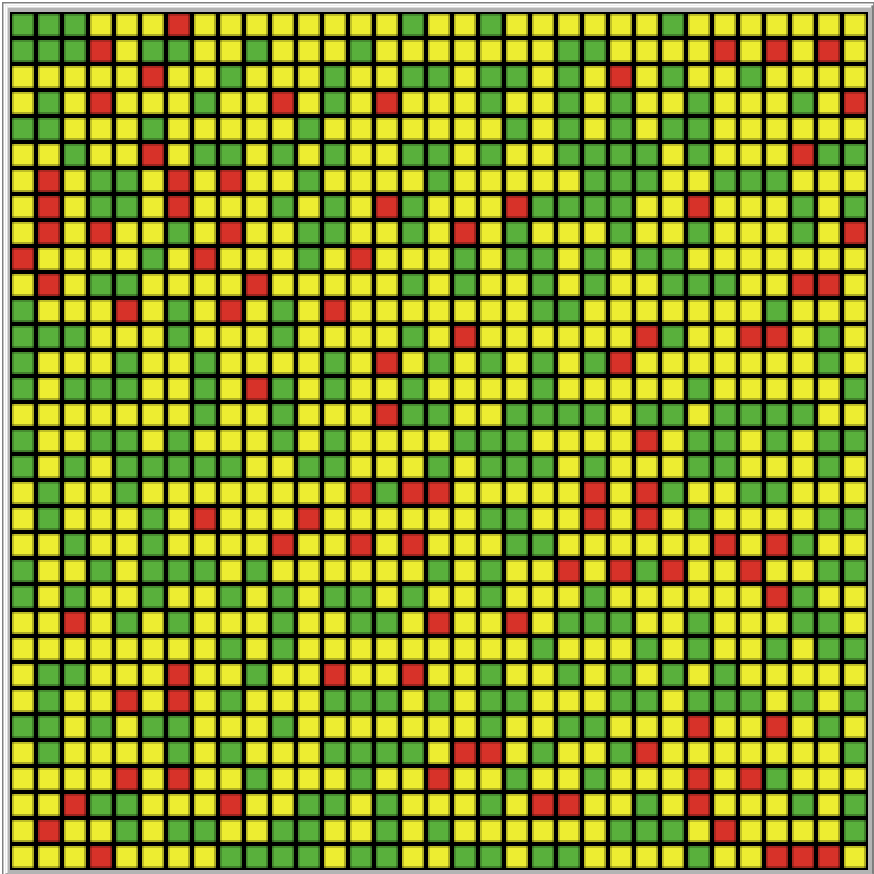
\includegraphics[width=6cm, height=6cm]{verystart}
	\caption{Beginning of a strike: working=green, willing=yellow, striking=red}
\end{figure}
\begin{figure}[htbp]
	\centering
	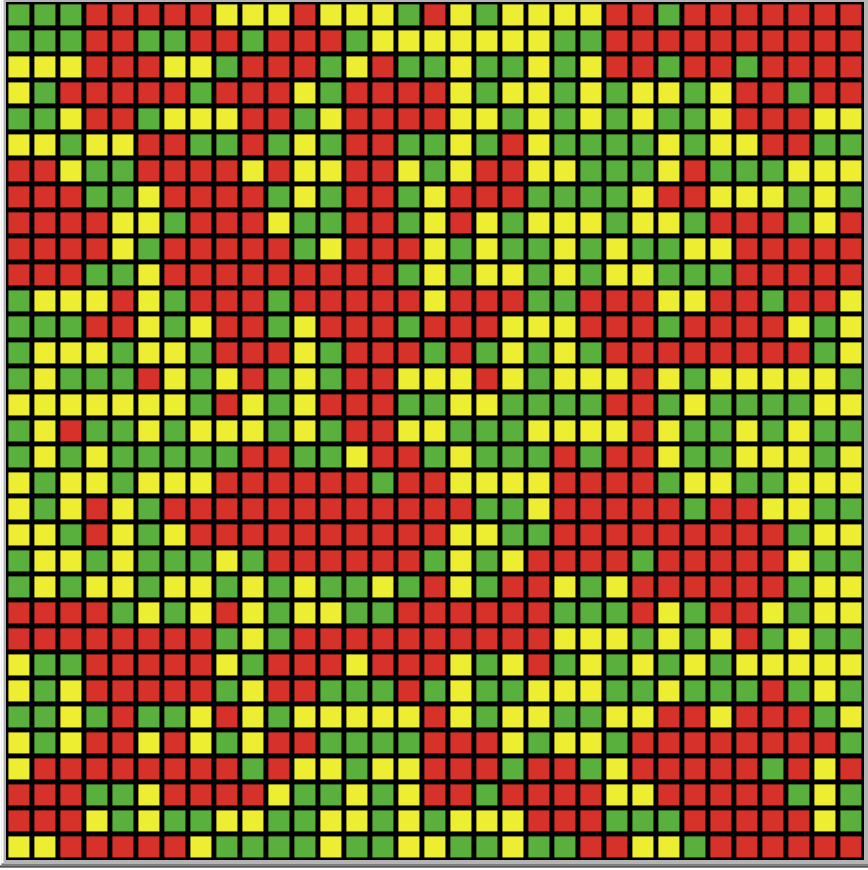
\includegraphics[width=6cm, height=6cm]{heavystriking}
	\caption{Heavy Striking}
	\centering
	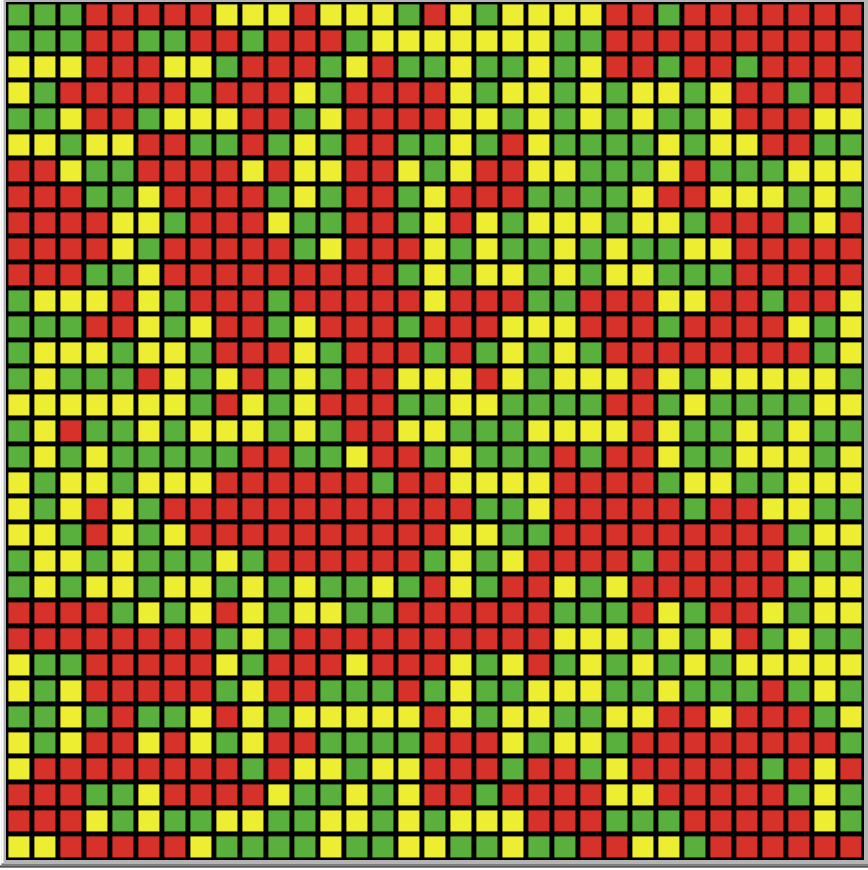
\includegraphics[width=6cm, height=6cm]{heavystriking}
	\caption{Less Striking}
	\centering
	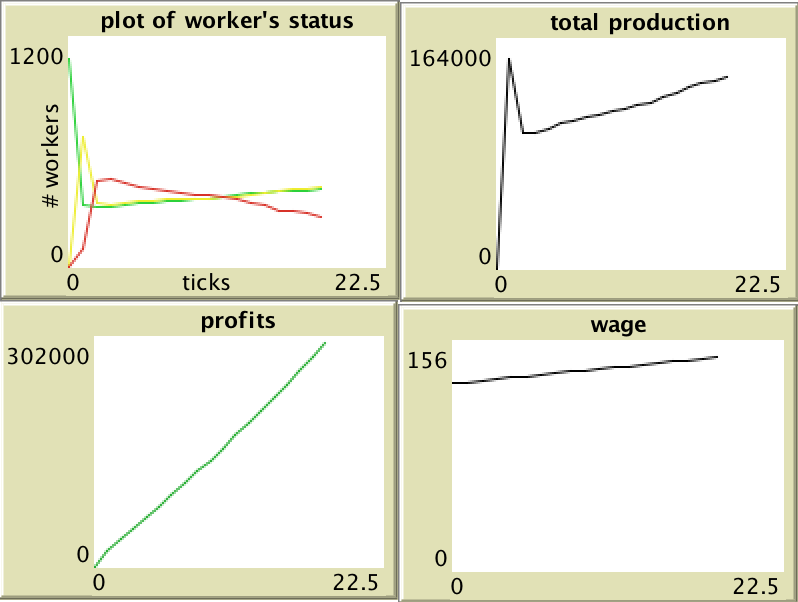
\includegraphics[width=6cm, height=6cm]{graph1}
	\caption{Graph of Figures 1-3}
\end{figure}
\begin{figure}[htbp]
	\centering
	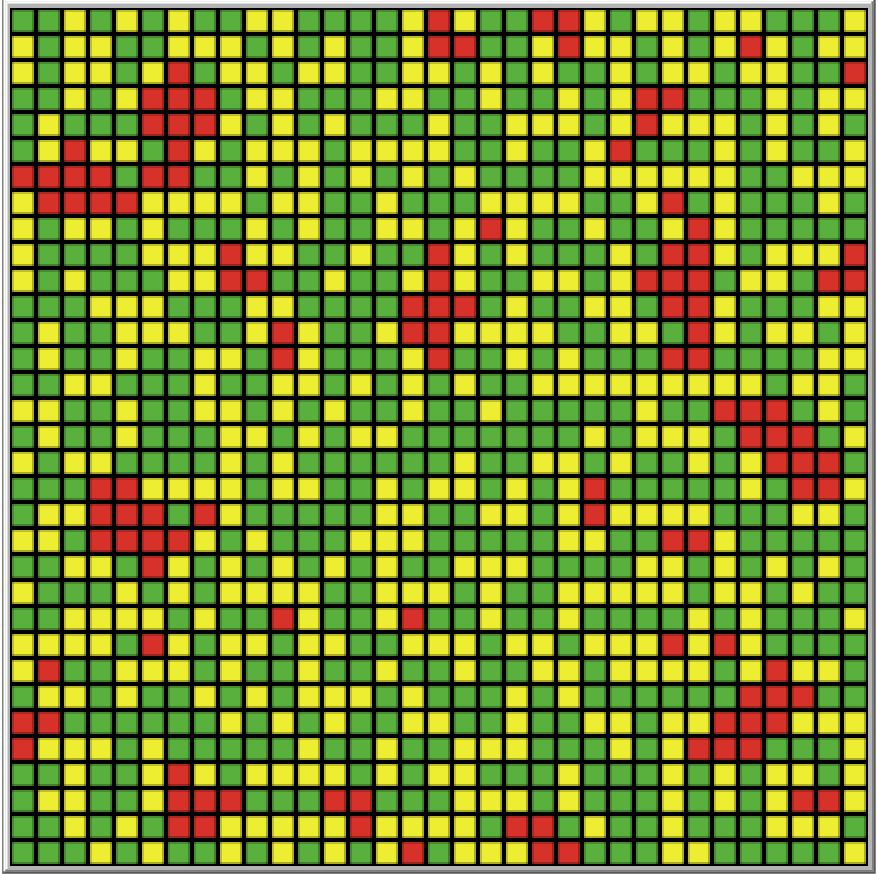
\includegraphics[width=6cm, height=6cm]{start}
	\caption{Mostly working after many iterations}
	\centering
	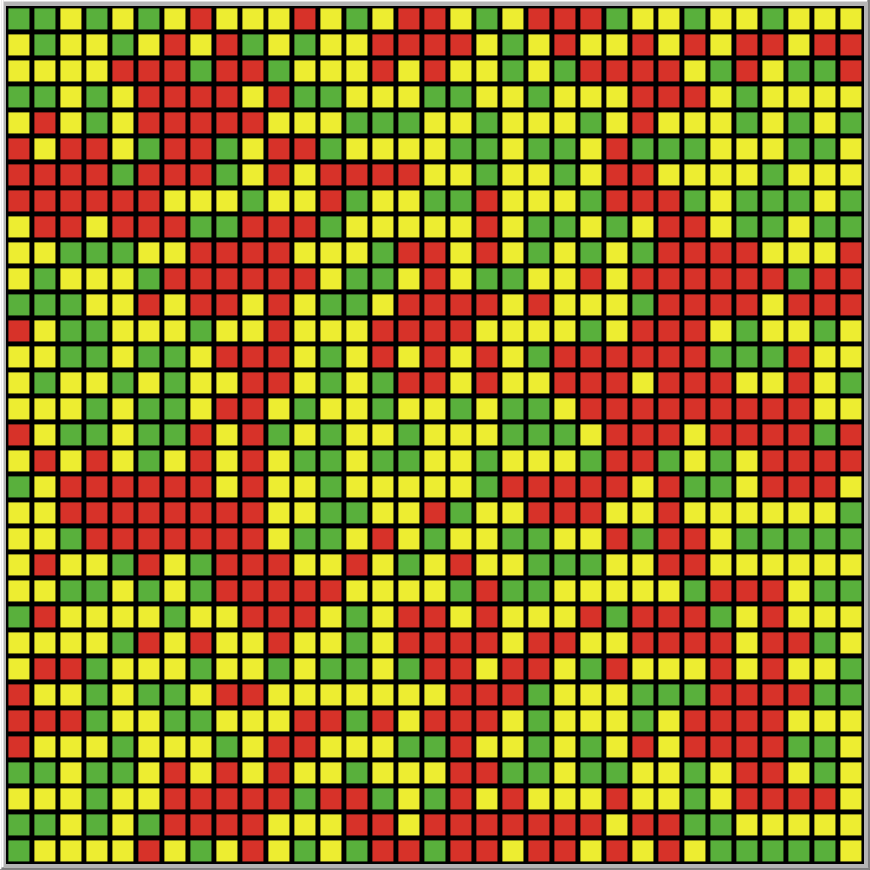
\includegraphics[width=6cm, height=6cm]{middle}
	\caption{Strike spreading}
	\centering
	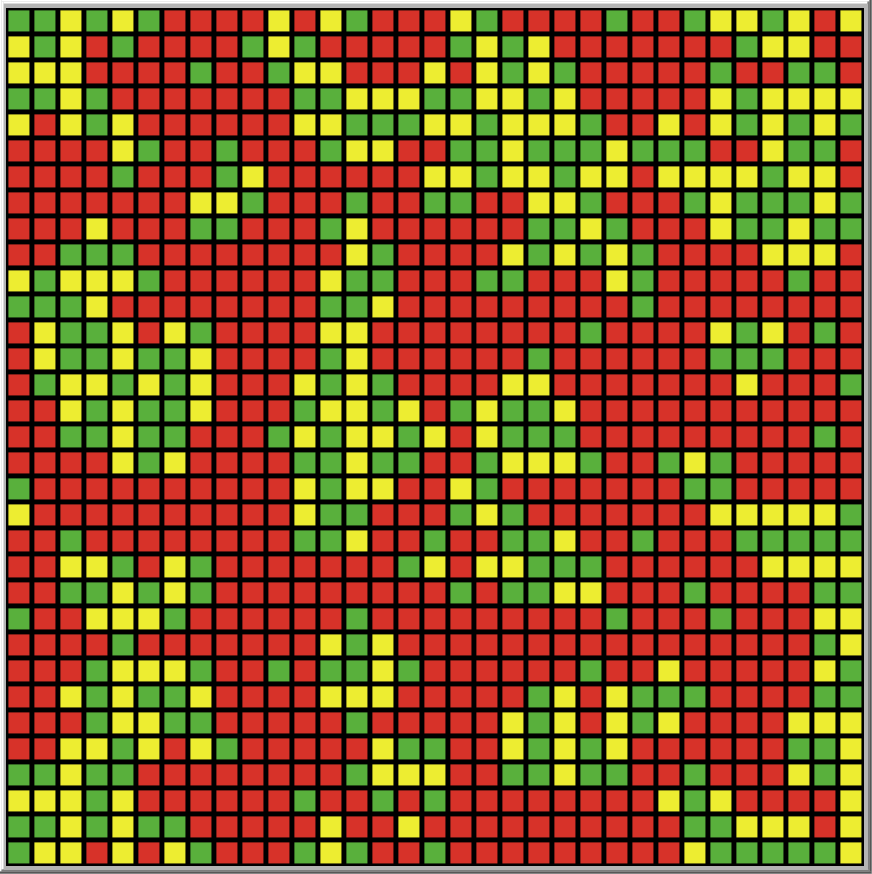
\includegraphics[width=6cm, height=6cm]{end}
	\caption{Intense spreading and islandization of working groups}
\end{figure}

\begin{figure}[htbp]
	\centering
	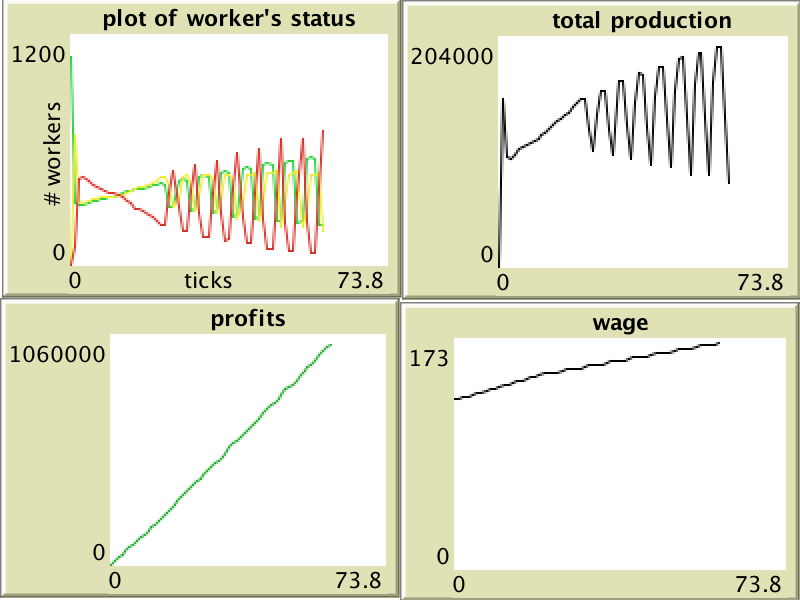
\includegraphics[width=6cm, height=6cm]{graph2}
	\caption{Graph of Figures 5-7}
	\centering
	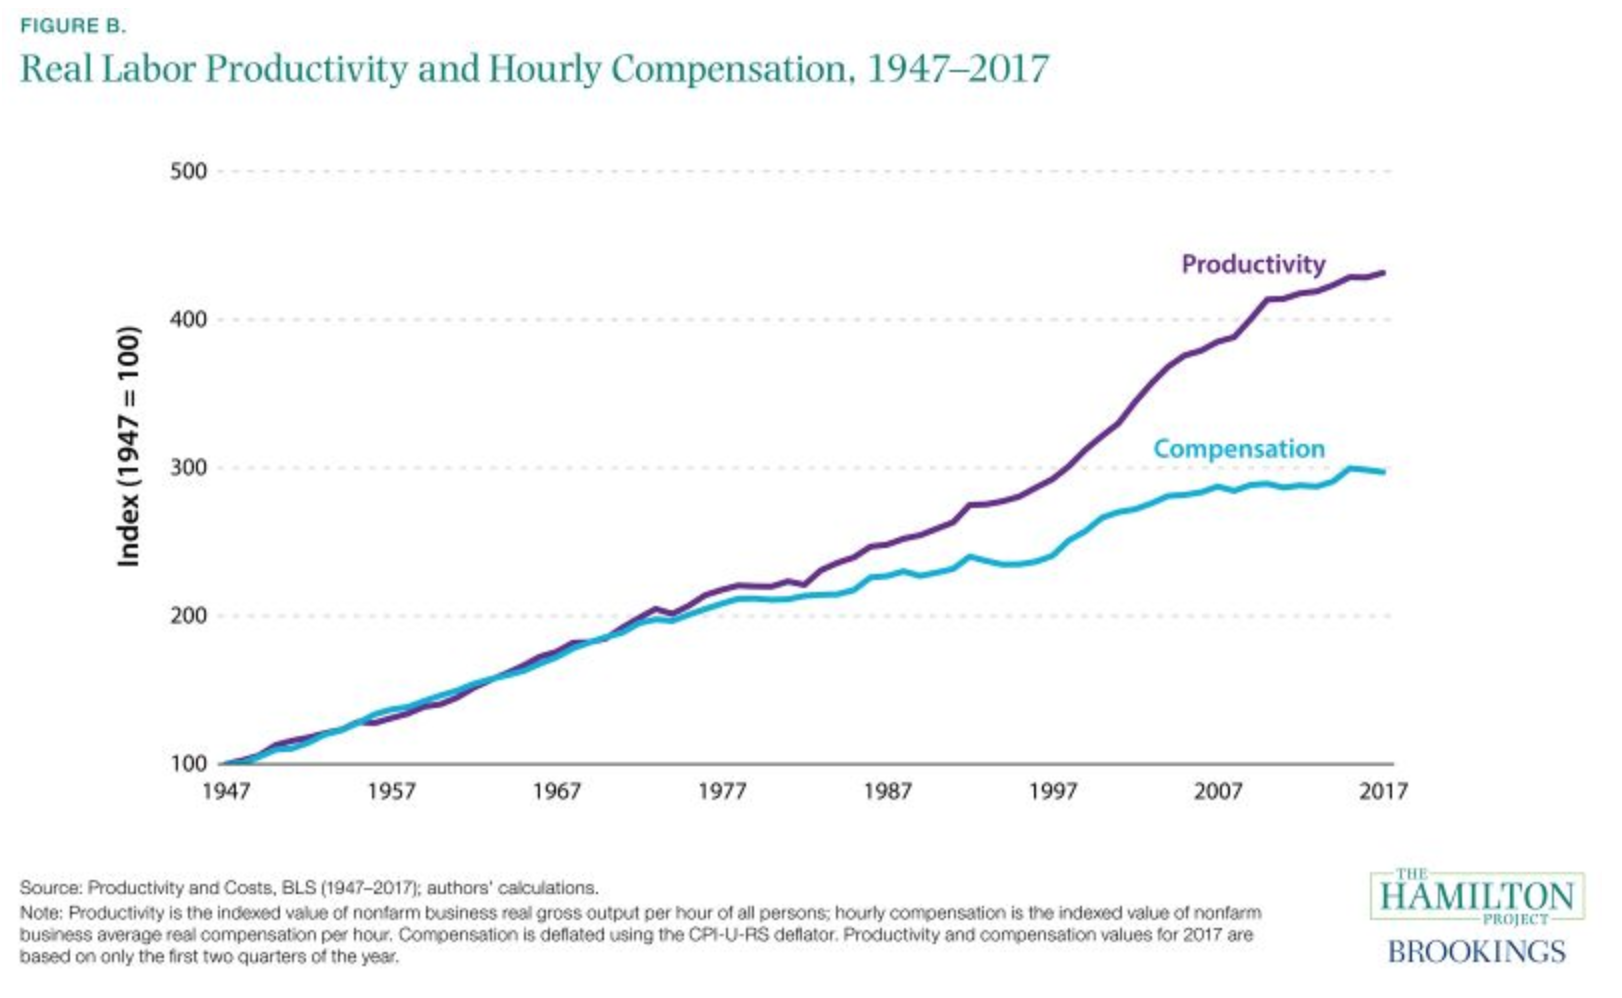
\includegraphics[width=10cm, height=6cm]{brookings}
	\caption{Brookings Institute Findings}
\end{figure}

\newpage


\section{Works Cited} \hrulefill

Shambaugh, Jay. "Thirteen Facts about Wage Growth." Brookings Institute, 25 Sept. 2017,
\qquad www.brookings.edu/research/thirteen-facts-about-wage-growth/. Accessed 8 Nov. 2018. \\

Proto, Eugenio. Are Happy Workers More Productive. IZA World of Labor. \\

Eaton, Curtis. "The Worker and the Profitability of the Strike." ILR Review, vol. 26, no. 1,
\qquad Oct. 1997. \\

Sugden, Robert. "Credible Worlds: the Status of Theoretical Models in Economics." Journal  
\qquad of Economic Methodology, vol. 7, no. 1, 2000. \\
     
     
Sugden, Robert. "Credible Worlds, Capacities and Mechanisms." Erkenn, 2009.  


\end{document}
